\documentclass{article}
\usepackage[utf8]{inputenc}

\title{Blockchain for manufacturing \\
 A practice for using blockchain \\
 on ESP32 microprocessor}
\author{WANG, Yuqiang \\ PANG, Sui \\ \url{https://github.com/Beck-Sisyphus/blockchain_on_esp32}}
\date{December 2017}

\usepackage{natbib, graphicx, csquotes, epigraph, listings, url, textcomp, gensymb}
\usepackage{amsmath,geometry,amscd,amssymb,verbatim,enumerate,mathrsfs,graphicx,CJKutf8,color,scalerel,stackengine,xcolor,polynom, geometry}
\usepackage{float, subcaption}
\DeclareGraphicsExtensions{.png}
\renewcommand{\familydefault}{\rmdefault}

\begin{document}

\maketitle

\section{Introduction}

    The blockchain is a distributed database that maintains a continual growing list of records called blocks secured from tampering and revision.\citep{narayanan2016bitcoin} Previous summary to implement the blockchain technology in the Internet of Things is extensively analyzed.\citep{christidis2016blockchains} Adding on top of cryptographic principles and technics including zero-knowledge proof, we have seen a few opportunities in the industrial robot industry.

    In the automation industry of Japan and Europe, only two parties are involved in building an assembly line, the industrial robot companies who seal the robots, and the manufacturing companies who use them. However, the industry is less monopolized in China, and there usually multiple parties involved, and figuring out responsibility in a malfunction situation is hard. If a manufacturing company purchases the mechanical robot arm body and the electrical controller from separate companies.

    \subsection{Application Scenes}
    For instance, the robot arm from Capek Robotics and the electrical controller from Googol Tech, when malfunctions occur, it is hard to analysis if it is a mechanical, electrical, or software error. In a situation like this, the raw data from the robot sensors are required for analysis to determine the reliability, yet the manufacturing company was willing to offer or analysis these data, worrying a leak on the critical manufacturing process. The manufacturing company will usually blame the controller company first, and ask the latter for compensation. At the same time, the controller supplier will worry if the data is tempered for more compensation. Hence a need is created for the controller supplier either to deploy a zero-knowledge proof to the manufacturing company that it is not their fault without showing them the method or to build a private chain network for sharing these data with a trusted record and a lower maintenance cost.

    Currently, most of the blockchain application we have seen are developed on commercial electronics. However, these electronics are not widely accepted in the industry for consideration on cost, power consumption, and electromagnetic compatibility. We used a computational limited microprocessor ESP32 to fit the need of the industry and deployed a blockchain for sharing information.

\section{Methodology}

    \subsection{Hardware Introduction}\label{sec:hardware}

    \begin{figure}[h]
      \centering
      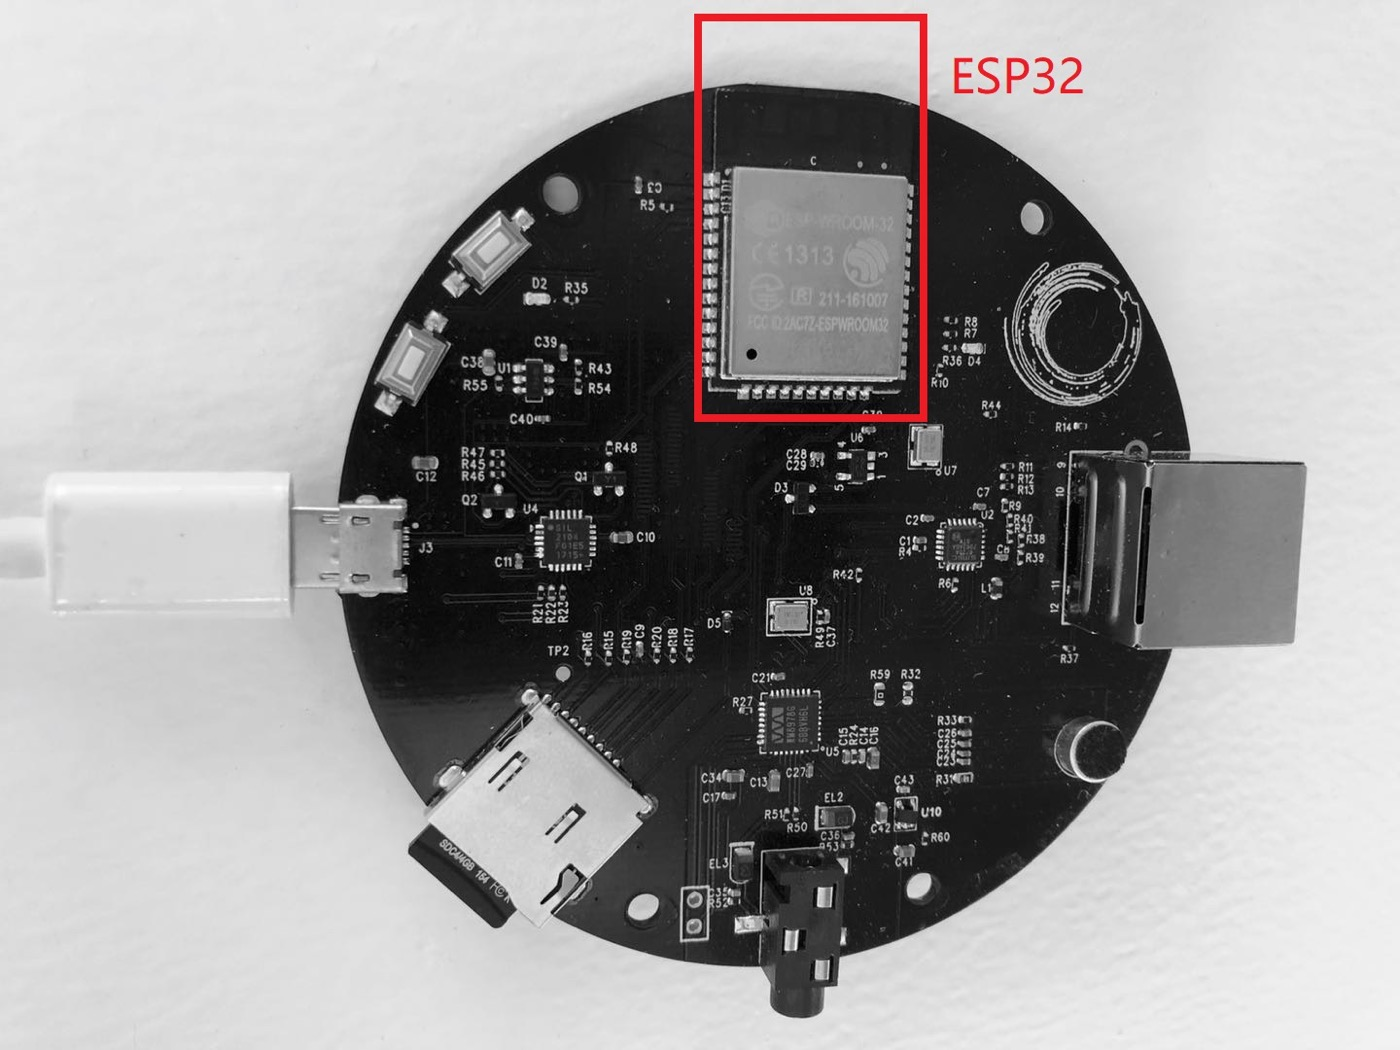
\includegraphics[scale=0.2]{esp32-circle.jpg}
      \caption{ESP32-circle module}
      \label{fig:espCircle}
    \end{figure}

    We choose the ESP32 microprocessor from Espressif Systems for its hardware level integration for SHA-256 function and common wireless communication protocols. The specification of the board is followed: \citep{espressifGithub}
    \begin{itemize}
      \item Xtensa Dual-core 32-bit microprocessor, running at 240MHz
      \item 448 KByte ROM
      \item 520 KByte SRAM
      \item 4 MBytes Flash
      \item Bluetooth 4.2
      \item Wifi 802.11 n(2.4GHz)
      \item SHA, AES, RSA, RNG Accelerator
    \end{itemize}

    With all these hardware level support, each esp32 node can connect to wifi automatically and connect with its neighbor through AP or even Ethernet through some protocols. With a Bluetooth module, the esp32 node also can detect its physical neighbors when needed. In order to simplify our processing difficulty, we use a trustable development board of ESP32 named ESP32 circle bought from Taobao. \citep{whyengineer} The photo of this board is shown in Fig.  \ref{fig:espCircle}:

    The major four challenges we faced are the hashed blockchain data structure, the flash memory management, web server and HTTP requests, and over-the-air firmware flash. The first three challenges are the core blockchain problem, while the last one is a design choice for implementation and demonstration. To understand and implement the blockchain from an engineering perspective, we decide not to utilize an existing platform, but to build a blockchain from scratch. The blockchain we build are simplified and weak in scalability but have all the core functionality nonetheless.

    \subsection{Simple Blockchain Design}
        In order to establish this blockchain system, we designed a simple blockchain system without proof-of-work as our first version.
        Let us introduce some upper-level structure of this system first. In this simple system, there is one special node (PC server) and more general node (ESP32). The function of the special node is providing new blocks, whole chain and the binary file (firmware) when requested by general ESP32 nodes.
        The flow chat in fig. \ref{fig:flowchart} of how a general ESP32 node works:

        \begin{figure}[h]
          \centering
          \includegraphics[scale=0.6]{flowchartNetwork.jpg}
          \caption{the flowchart of work structure of a general node}
          \label{fig:flowchart}
        \end{figure}

        When the general node start working it will firstly send a request for the special node, if succeed, it will check if its firmware version is the latest one. After checking process, it works as a web server that will provide its latest block, whole chain, and firmware data when getting requests from other nodes that list it as their neighbor. If the general node does not get a response from the special node, it will send a request to its neighbor one by one and get the longest chain it can request through all its neighbor list. If no node response to this general node, it just keeps its own chain and serves as a web server.
        The checking process is shown as Fig. \ref{fig:flowchartChecking}.

        \begin{figure}[h!]
          \centering
          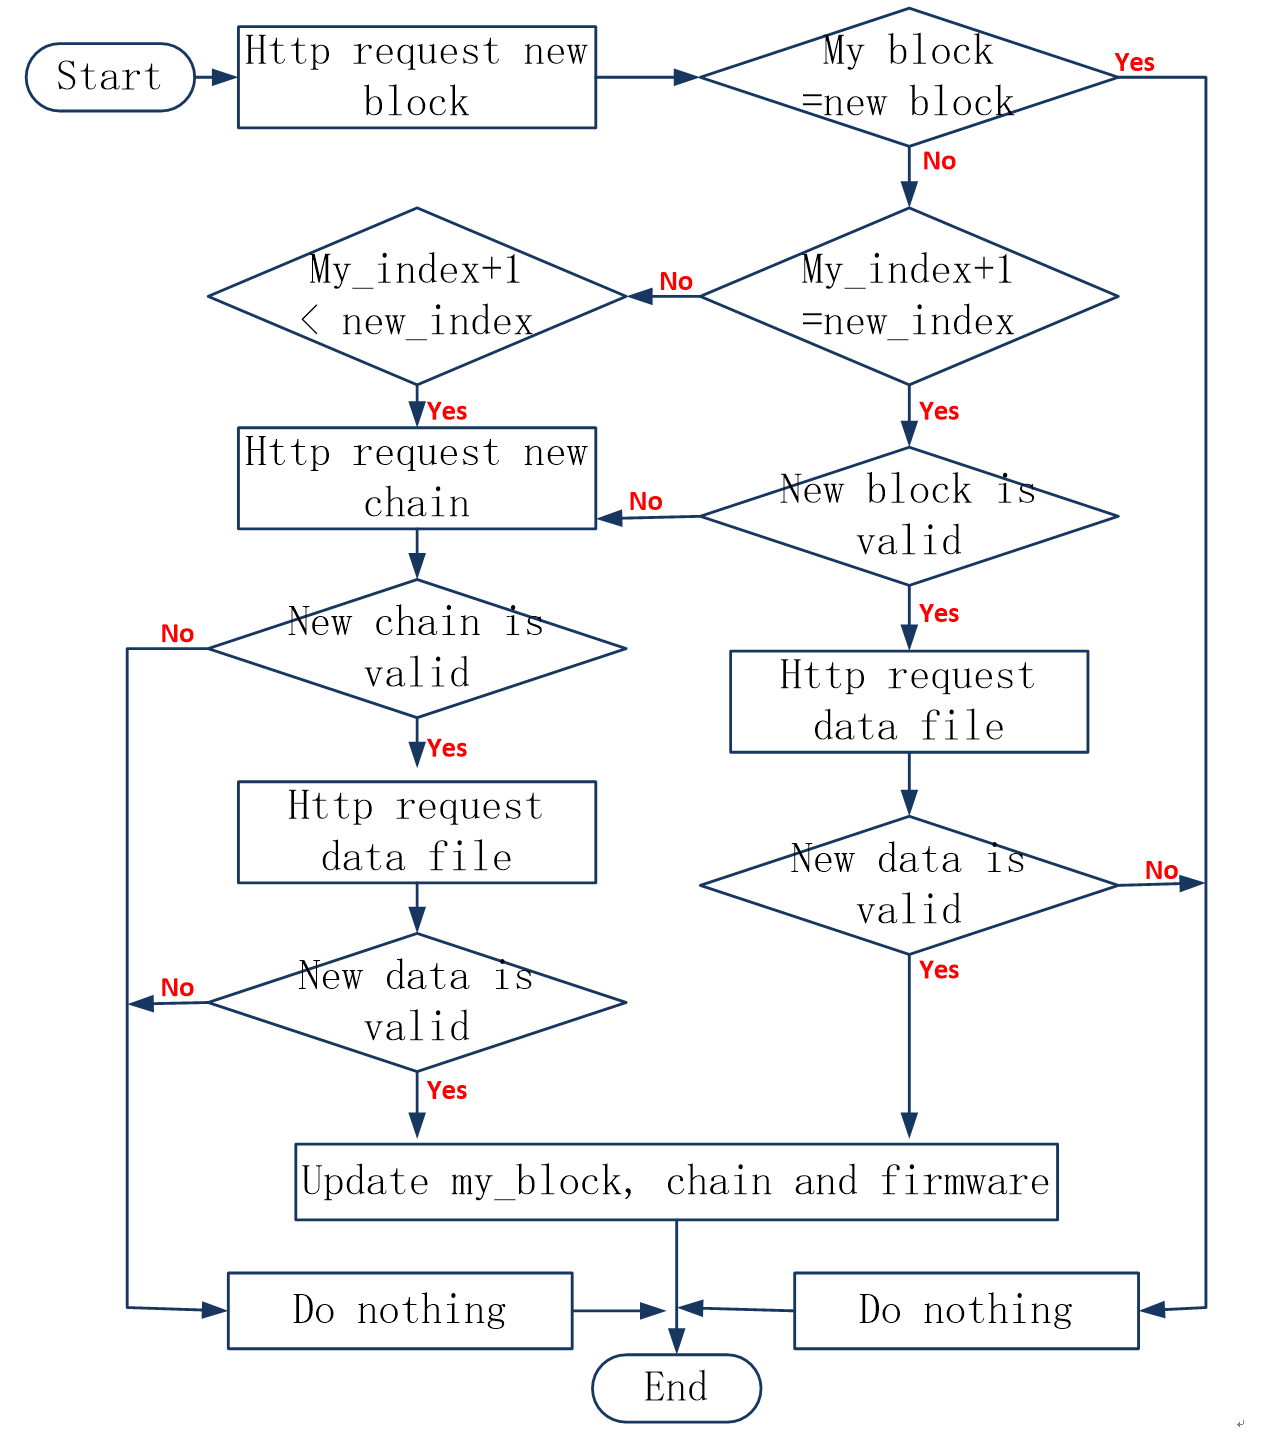
\includegraphics[scale=0.2]{flowchartChecking.jpg}
          \caption{the flowchart of checking process}
          \label{fig:flowchartChecking}
        \end{figure}

        The checking process flowchart illustrates how a node checks if it gets a valid block. After it gets a new block from another node, it will first compare its own latest block with the new block, if they are the same, which means the firmware is the latest version and no need to change. If these two blocks are different, one possibility is the new block is the next block of the local chain when the index of the new block is the index of the local latest block plus one. So after verifying the new block and new data file, this node will update all files in its flash. The other possibility to update firmware is when the index of the new block is larger than the index of the latest block and both the data file and the whole requested chain are valid. Otherwise, do nothing.

        \subsubsection{Block Design}
        The block is stored in an array in fixed memory address in the array of 8 bit unsigned integer with the following structure structure:

        \begin{itemize}
          \item index
          \item timestamp
          \item the hash value of the .bin data
          \item the hash value of the previous block
          \item the hash value of the current block
        \end{itemize}

        The hash function we choose is SHA-256, a subclass of the Secure Hash Algorithm, a reliable hash function which is proved by Bitcoin system. We utilize the hardware SHA-256 solver on the ESP32 chip for non-blocking thread calculation. All items in the block are stored in the array of an 8-bit unsigned integer for the ease to integrate with the SHA-256 solver.

        \begin{figure}[h]
          \centering
          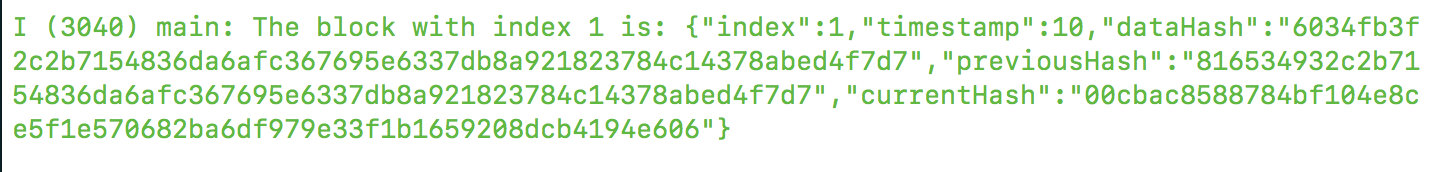
\includegraphics[scale=0.5]{lastest-block}
          \caption{screen shot of one block}
          \label{fig:lastest block}
        \end{figure}

        For communication and operations, the block structure parsed into the JSON object, shown in the Fig. \ref{fig:lastest block}. The data is stored in cJSON linked list object in RAM, and stored in pre-allocated memory address in flash.

      \subsubsection{flash memory management}
          In this project, we decide to use the one chip flash as our chain and data storage driven by a lot of reasons. According to Section \ref{sec:hardware}, we know our chip has a 4M flash and the size of firmware is always less than 100Kbyte. So the space of flash is enough to store a small size block-chain and a new firmware. What is more, it is easier to read and write data on flash than on a TF card. Another important reason is the data stored in flash can be changed by the program and will not be erased after power down.

          The flash memory on the chip is partitioned by the official guide of ESP32 and we can use the standard library to utilize a partition table to create different partitions for data management. The partition table on the chip is handcrafted, and every partition can have different property relative to its type.

          \begin{figure}[h]
            \centering
            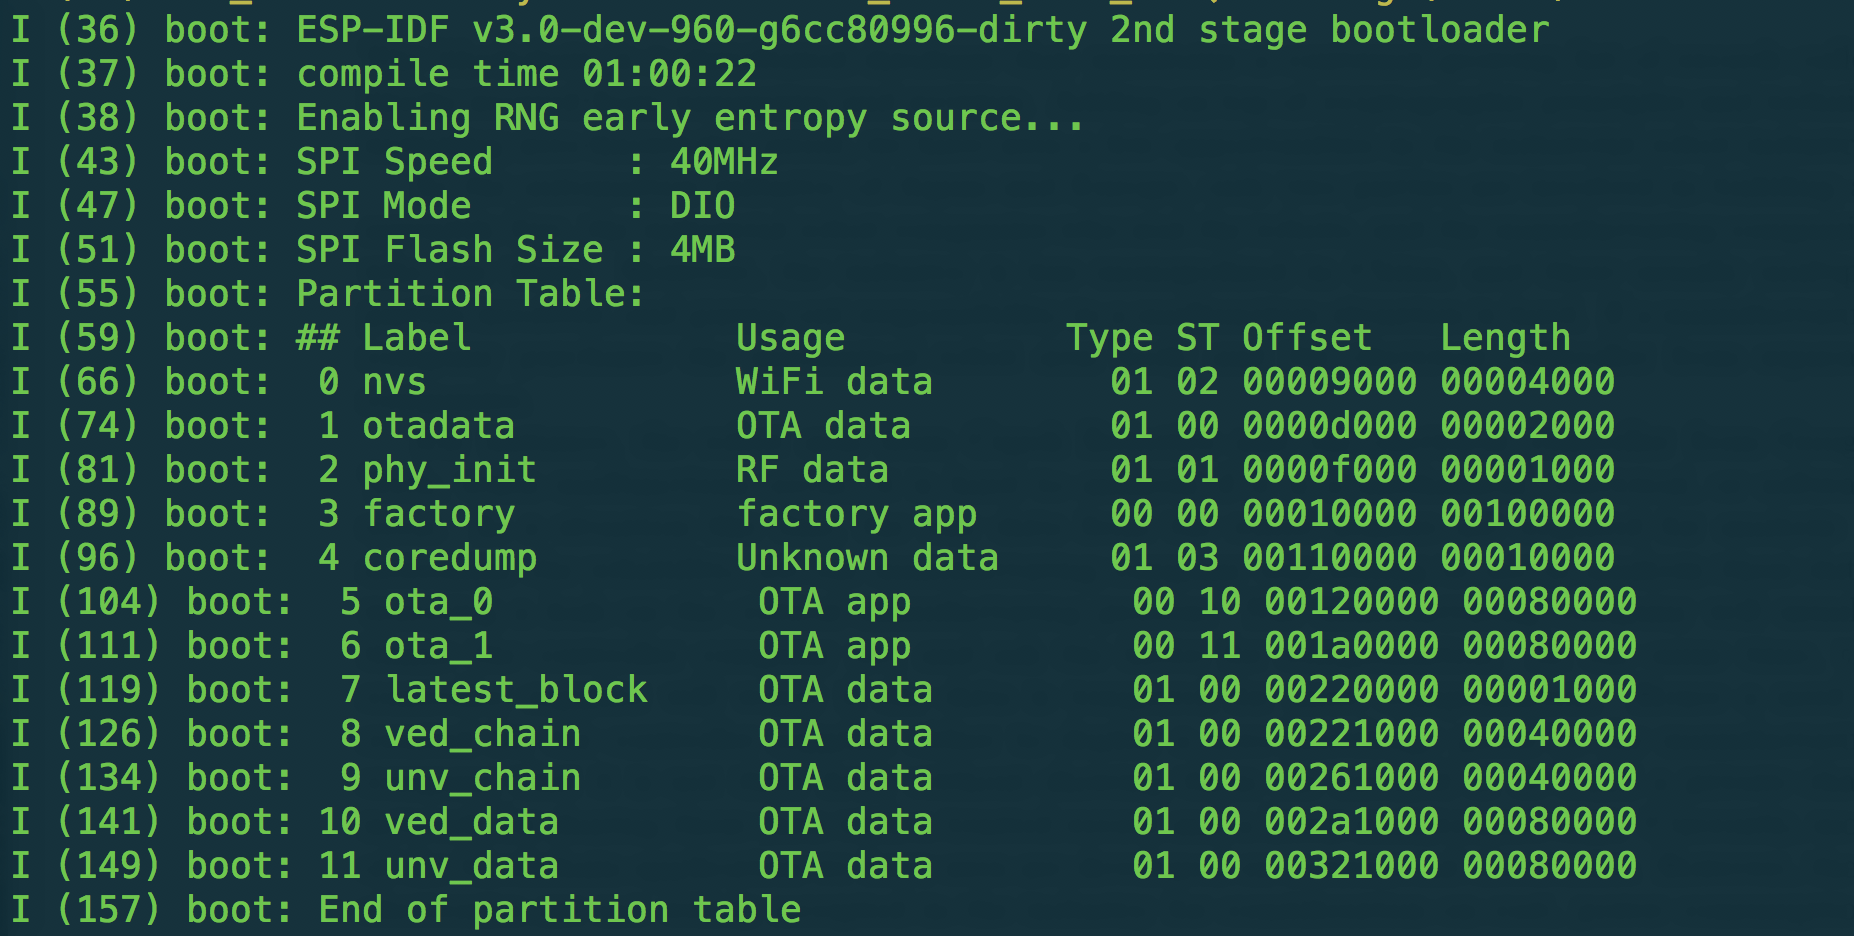
\includegraphics[scale=0.3]{partitionTable}
            \caption{screenshot of printed initialized partitions}
            \label{fig:partition table}
          \end{figure}

          As we can see there are 12 partitions in total. Partition 0,1,2,4 are for specific use; partition 3 is designed for factory program that will not change after the chip sold out; partition 5 and 6 are designed for the firmware that can update later on. Partition 7 to 11 is designed for store the block and firmware information. In order to save the limited Flash space, we will not store previous firmware data. Only the verified current firmware will be stored in partition 10 (verified data partition).

          The partition 8 verified data is used for storing verified data, starting from genesis block with increasing block index. The block size is a constant, which means we can find one block in verified data partition by its index. However, we cannot know how many blocks is in the chain if we do not know the index of the latest block. Thus we create a small partition to store the latest block, latest\_block partition.

          We have two pairs of partitions for verified and unverified chain and firmware data. Because the size of chain and firmware data may be too large compared to the size SRAM (520 Kbyte) and it is dangerous to just store them only in SRAM, even we just use them for a while.

      \subsubsection{validation}
          When a new block or a new firmware binary arrived, they are validated by checking their hash. Follow the tutorial for a simple block chain\citep{simpleBlockchain}, When a block arrived, its index, its block hash, and the previous hash with the next hash are verified with the current chain. If a block hash collision appears, a complete chain will be requested. Once all verification passed, the data binary will be requested and verified with the latest block data hash.

         The genesis block previous hash is a hardcoded random value, and its data hash is generated by the factory code. The data hash for each block is the hash of the running firmware binary. And to generate the hash pointer, all the data on the block will be hashed.

    \subsection{web server and http requests}
        A simple web server with hardcoded IP address is written to the chip for access the upcoming data. The data are transmitted through web socket in JSON format.

        \subsubsection{socket}
        A socket is created once a node wants to send or receive data. In this system, every node will have its own IP address and the socket address is defined by both IP address and port address.
        Thus the content of the neighbor list is the socket address (IP and which port of the neighbor can serve as a web server) of its neighbor.

        \subsection{HTTP protocol}
        For the things that transferring through sockets, HTTP protocol is used to let one node connect to PC and other nodes.
        Limited by the computational power, it is not possible to use a complete standard HTTP protocol in ESP32. We designed several specific HTTP request and response functions for a determined purpose.

	\subsection{request part}
        For request part, we designed three functions that can request data from a PC server or an ESP32 web server. The three functions are:
        \begin{enumerate}
            \item http\_request\_latest\_block
            In this function, a node at first will sent a GET request whose URL is IP\: port/latest\_block.c. Then it gets the HTTP response with a block of JSON output format string in its body part. At last, the function needs to store the body part and store it in the variable new\_block.

            \item http\_request\_whole\_chain
            The URL of the GET request of this function is IP: port/chain.c. The response body it gets is the whole chain. This function will directly store the whole unverified chain to unv\_chain partition package.

            \item http\_request\_data\_file
            This function is quite similar with the last one. The URL of its GET request is IP:port/file\_name.bin. This function store the whole body part of the HTTP response package by package to unverified data partition (unv\_data).
        \end{enumerate}


    \subsection{web server part}
        After all checking process, one node will start its server duty to send HTTP response when requested. There are three response functions corresponding to the request functions.
        \begin{enumerate}
            \item http\_response\_latest\_block
            The function is called by URL /latest\_block.c and will return HTTP1.0 200 OK, a simple header with Content-Type and Content-Length and a body part that contain the latest block read from latest\_block partition.
            \item http\_response\_whole\_chain
            The function is called by URL /chain.c and have the whole chain as its body part, which is read from verified chain partition (ved\_chain).
            \item http\_response\_data\_file
            The function is called by URL /file\_name.bin and with its body part read from verified data partition (ved\_data).
         \end{enumerate}


    \subsection{over-the-air firmware flash}
        Over-the-air programming is the method to distribute new firmware through wireless communication Wi-Fi. In our platform, a new binary image is saved through the blockchain in the flash for subsequent execution on next restart. The program will first verify the chain and the binary hash of the incoming firmware binary. The verified application binary will be flashed on board.

    \subsection{security consideration}
        As this simple blockchain is too weak that cannot protect itself from evil attacks. For example, without proof of work, it is extremely easy to create a long chain that can replace the chain on another node. Thus before putting the system into production use, a zero-knowledge proof is needed to increase the safety of the whole system.
        The point is quite simple: Add a signature item on block structure. The people or company that have the right to update the firmware will have a key, with this key they can create the valid signature of any block. In other words, they can sign this block. With this signature, node believes the block is published by the real special node.
        On the other side, every time when a node verifying a block, they also verify the signature to avoid malicious long chain attack.

\section{Experimental evaluation}
    We start this project quite early, we selected ESP32 as the chip we want to use for this project in October, and start to establish the toolchain for it and write hash function on it. We get a solid understanding of the upper level of how blockchain works in class, but it also takes time to write real C function to hash or verify objects.
    However, later on we find without any background of network really troubles a lot. What is the worse, there is no lots of ESP32 examples for HTTP request and even less for the web server.
    Even faced with all these difficulties, we still get a lot of progress. The source code is opensourced at Github on the first page of this report.
    \subsection{current states for the blockchain}
    \begin{itemize}
        \item block structure: The structure and communication are implemented.
        \item validation functions: the verification for chain append is implemented. Data hash verification not implemented.
        \item replace chain: not implemented
        \item chain storage: The storage in cJSON object and in flash are implemented.
    \end{itemize}

    \subsection{block and firmware storage}
    A complete library of reading and writing latest\_block, read any block on the chain, transfer new chain from unv\_chain partition to ved\_chain partition is finished and well worked. The data will keep even after we flashing new programming in it.

    \subsection{HTTP web server}
    \subsubsection{HTTP web server in PC node}
    In order decrease the workload of the whole system and we have no more time to learn Nodejs we select to use the simplest method: write the information of latest block and chain into latest\_block.c and chain.c file and use command “python -m SimpleHTTPServer 8070” to create a web server in PC node.

    \subsubsection{HTTP request in ESP32 node}
    The three request functions were written and they can successfully get data from PC node and write them to flash or store them in a variable.

    \subsubsection{HTTP web server in ESP32 node}
    The three response functions were also written and when we use a browser to connect the node it will send correct HTTP response. We use a free web debugging tool Fiddler to check the raw data. The body part is the same are the response sent by the PC node.
    \begin{figure}[h]
      \centering
      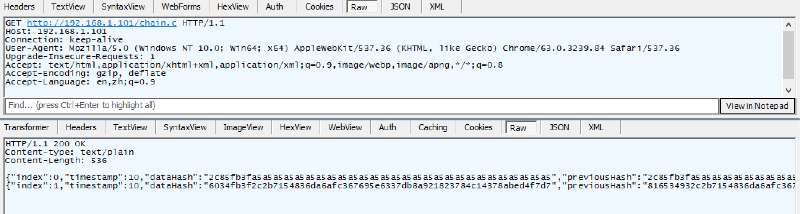
\includegraphics[scale=0.4]{package.jpg}
      \caption{screen shot of the a HTTP request from PC and the response from a ESP32 node}
      \label{fig:partition table}
    \end{figure}

    \subsection{communication between two node} \label{sec:communication}
    After the testing of communicating of the ESP32 node and PC node. We started the communication of two ESP32 nodes. Now we can send the latest block form a server node to a request node. In terms of the other two pairs of functions, it is sure the requesting node received something but seems very strange.
    What is more, we also have a problem with when we send the second request the server also working on the first one and cannot respond the second request while ESP32 to ESP32 connecting. (The web server works very efficient when we use browser on our phone to connect it and need a longer time to finish response when we use browser in our PC.)


\section{Future Plan}
    \subsection{combine}
    After solving The problem in Section \ref{sec:communication}, we can combine every part together and get a simple workable blockchain system with one PC and several ESP32.
    \subsection{over-the-air firmware flash}
    Then we can add OTA firmware update part on the simplest blockchain system.
    \subsection{neighbor node list}
    In the simplest system we are establishing now, there is one special node (PC), two general nodes (A and B), for one general node it only has one neighbor. So, no neighbor list needed. But for a real system, a neighbor node list is needed.

\section{Limitation and Solution}
    \subsection{physical space limitation and Ethernet connect}
    In this project, the information is flowing under a Wi-Fi environment, which limits the physical space of the whole system. Fortunately, The ESP32 also can connect to Ethernet, which can solve the problem of remote connection from the node to node.
    \subsection{storage shortage and TF card}
    Consider the increasing size of chain, it is not too difficult to store all things in a TF card.
    \subsection{hash the binary on chip}
    Since in the embedded system, the binary that runs on the chip is much larger than the block, it is hard to send to the SHA-solver without running out of the space on RAM. For instance, our block is 102 bytes long, and when stored in cJSON, it is 268 bytes long, however, the binary to hash is 144 KBytes long. We need to utilize the flash memory in order to hash it.

\section{Conclusion}
    In this project, we have explored the several engineering collenges to build a blockchain application from scratch. We have implemented a mimimum size blockchain in an embedded platform without proof-of-work, and made half way on the board to board communication. The details about how to repeat the work please reference to the README file on our github project.

    We also appreciated the system and network engineering efforts the blockchain pioneers have put into a larger system like Bitcoin and Etherum. We realize that the blockchain technology is a system engineering, and requires multiple engineering discipline to work. We have just started, and hope to further explore this field.

\bibliographystyle{plain}
\bibliography{references}
\end{document}
